% \mychapter{3}{Testing}
\mychapter{4}{Results}

Using the previously derived stability criterion, we can now test what affect the different stabilisation types have on the backflow for different parameter values, and if they are able to attain the stability criterion. We will first begin by looking to the case where there is no added stability term and checking whether indeed the unstabilised backflow is causing there to be negative eigenvalues once discretised. Following this, the effect of the different stabilisations will be observed on the eigenvalues to see how easily they can be automated, which will give us the information needed in the next chapter where, if possible, the algorithms will be presented for the automation of the different backflow stabilisation method parameters.

\section{Testing environment}

In order to conduct our investigations, we will need some relatively general test case with which we can verify our analytic results. The tests that will be performed will be on a specific geometry, a representation of a tubular organ(vein, wind pipe, etc.) with a stenosis, which is a commonly occurring physiological problem, and thus a geometry which could often be encountered when solving the problems. The geometry will look as follows:\\
\begin{figure}[h]
\centering

\includegraphics[width=0.5\textwidth]{latex/Thesis/media/stenosis.png}
\caption{The geometry on which the tests will be performed\label{fig:testgeo}}
\end{figure}

where boundary conditions are specific on the top and bottom boundaries and an inflow term coming from the left boundary. The right boundary is the before mentioned natural boundary condition which is satisfied once a solution has been found. Appropriate values to the constants , such as viscosity and density, are given and a relatively high Reynolds number of 5000 is used as backflow effects are stronger with higher Reynolds numbers.
\includecomment{Add all the details about the test environment}

% \section{Results}



\section{Effect of different stabilisations}
Now we would like to observe what affect the different stabilisations have on the eigenvalues of \mathm{-B+S}. So we first select a time step in our simulation where backflow is occurring, and then look at what effect changing the parameters of our stabilisation methods has on the eigenvalues.

\subsection{No Stabilisation}
One of the first tests that would be important to conduct is to verify that our stability criterion is not attained in the presence of backflow with no stabilisation added. Thus just the eigenvalues of the discretisation of \mathm{- B} as defined in \autoref{eq:backflow} will be observed. What we would expect is that there are a few negative eigenvalues which would be responsible for the instabilities seen during the simulation and indeed in \autoref{fig:Nostabmulti} we see that it is indeed the case that there are negative eigenvalues for various times when there is backflow occurring. An interesting observation to note is that the eigenvalues change for each times step, which would make it nearly impossible to find a stable value for the parameters before the simulation except for the theoretically stable values.

\begin{figure}[ht]
     \centering
     \begin{subfigure}[h]{0.3\textwidth}
        \centering
        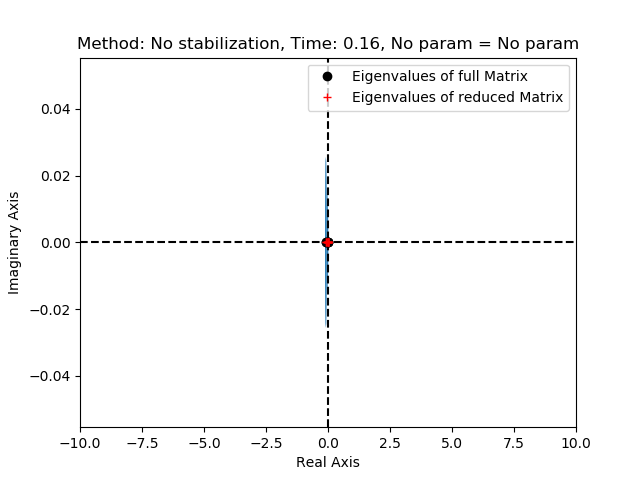
\includegraphics[width=\textwidth]{latex/Thesis/media/NoStab1.png}
        % \caption{Minimum and maximum eigenvalues\label{fig:VeloEig}}
     \end{subfigure}
     \hfill
     \begin{subfigure}[h]{0.3\textwidth}
        \centering
        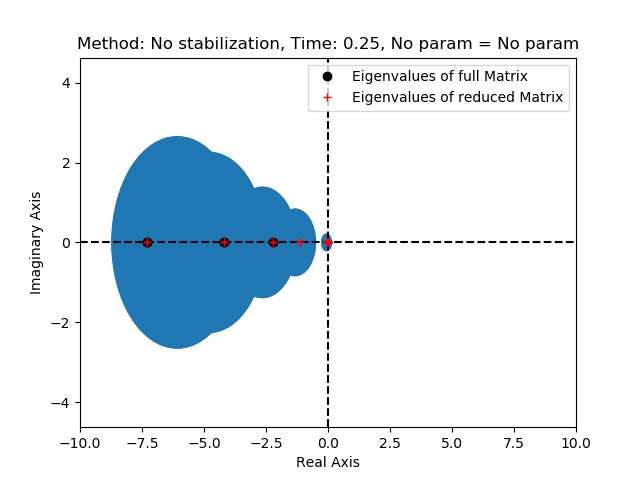
\includegraphics[width=\textwidth]{latex/Thesis/media/NoStab2.png}
        % \caption{Minimum eigenvalues\label{fig:VeloEigMin}}
     \end{subfigure}
     \hfill
     \begin{subfigure}[h]{0.3\textwidth}
        \centering
        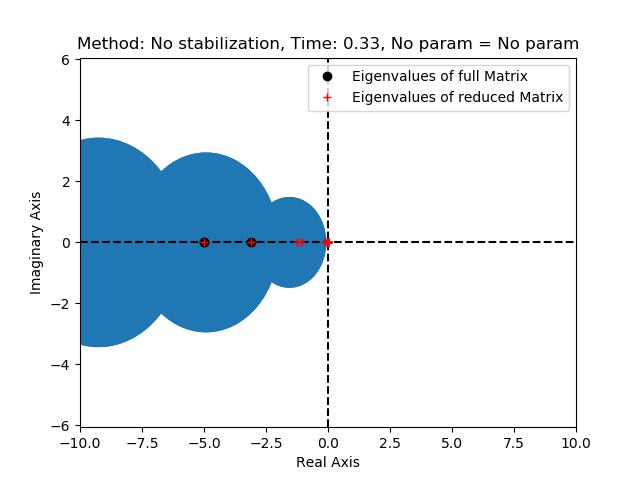
\includegraphics[width=\textwidth]{latex/Thesis/media/NoStab3.png}
        % \caption{Minimum eigenvalues\label{fig:VeloEigMin}}
     \end{subfigure}
        \caption{Eigenvalues for no stabilisation at different time steps}
        \label{fig:Nostabmulti}
\end{figure}

\includecomment{Include there a picture of the eigenvalues becoming negative with no stabilisation}

\includecomment{Also note something about how the flow changes at every time step so cannot select a single parameter before computation, besides 1, that guarantees stability}

\subsection{Velocity Penalisation}
The first stabilisation method which will be considered is the Velocity Penalisation method as defined in \autoref{eq:stabVeloPen}, and as noted before, this method has been proven to guarantee stability for a parameter value \mathm{\beta = 1}, so we would expect there to not be a negative eigenvalue for that \mbeta value. We first look to \autoref{fig:VeloEig} where we are looking at the maximum and minimum eigenvalues of the discretisation of \mathm{-B + S} \includecomment{Maybe here use a ref instead and before somewhere put -B +S since it will be used so much}as well as the difference between them.
\begin{figure}[ht]
     \centering
     \begin{subfigure}[h]{0.49\textwidth}
        \centering
        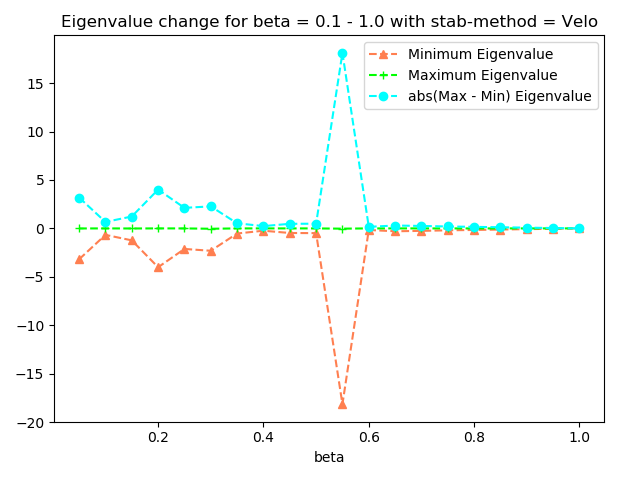
\includegraphics[width=\textwidth]{latex/Thesis/media/Beta_1_thru_0_velo.png}
        \caption{Minimum and maximum eigenvalues\label{fig:VeloEig}}
     \end{subfigure}
     \hfill
     \begin{subfigure}[h]{0.49\textwidth}
        \centering
        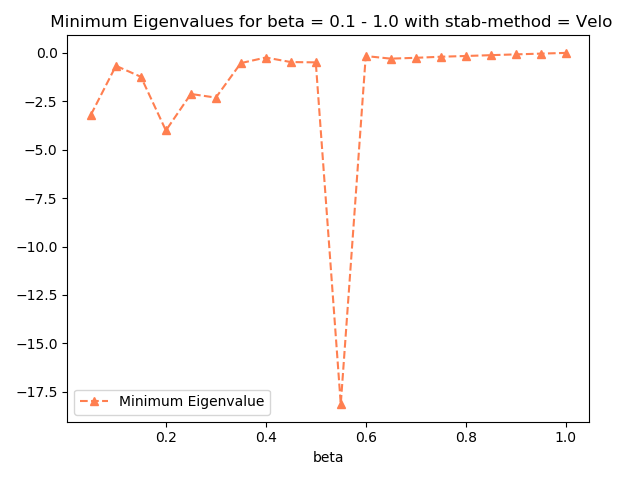
\includegraphics[width=\textwidth]{latex/Thesis/media/Beta_1_thru_0_velo_min.png}
        \caption{Minimum eigenvalues\label{fig:VeloEigMin}}
     \end{subfigure}
        \caption{Eigenvalues when using the Velocity Penalisation Stabilisation for various \mbeta's}
        \label{fig:VeloEigmulti}
\end{figure}
What can first be noted from \autoref{fig:VeloEig} is that when \mbeta~is less than one, the minimum eigenvalue appears to become negative. To see this in greater detail we can look to \autoref{fig:VeloEigMin} where we only plot the minimum eigenvalue as a function of \mbeta. This Figure more clearly shows that if we decrease \mbeta lower than one, then it could be possible for there to be a negative eigenvalue. This presents quite a problem for the basic automation since it means that if we want to consider values for \mbeta~lower than 1, we would need to include other terms which also help counteract the backflow instabilities, thereby increasing the computational cost of the automation.

\subsection{Tangential Penalisation Max}
The second stabilisation method to be considered is the Tangential Penalisation Max method as defined in \autoref{eq:stabTangPenMax} which has also been analytically proven to be stable when its parameter \mgamma~is equal to the Poincar\'{e} of the domain. Thus we would expect that if we make \mgamma~sufficient large, we will no longer observe any negative eigenvalues and thus would have stability. We first look to \autoref{fig:TangMaxEigLow} where as before the maximum and minimum eigenvalues of \mathm{-B+S} has been plotted and also to \autoref{fig:TangMaxEigLowMin} where only the minimum eigenvalue has been plotted as a function of \mgamma. From this range of \mgamma's we cannot conclusively make any sort of statement about if the eigenvalues are now all becoming positive, so thus we look to \autoref{fig:TangMaxEigHigh} and \autoref{fig:TangMaxEigHighMin} where we consider a much larger range of \mgamma's and now we clearly see that the minimum eigenvalue is being made positive if gamma is made large enough. Thus, just by using the stabilising term we are able to satisfy the conditions of the stability criterion, without relying on any other terms to aid with fighting the backflow.
\begin{figure}[ht]
     \centering
     \begin{subfigure}[h]{0.49\textwidth}
        \centering
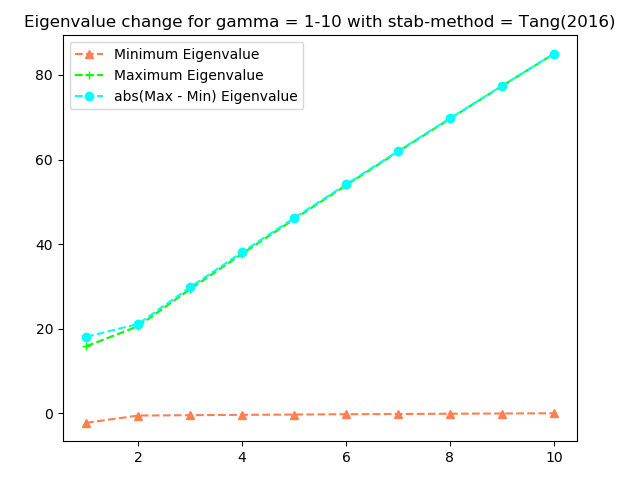
\includegraphics[width=\textwidth]{latex/Thesis/media/Gamma_1_thru_10_tang(2016).png}
\caption{Minimum and maximum eigenvalues\label{fig:TangMaxEigLow}}
     \end{subfigure}
     \hfill
     \begin{subfigure}[h]{0.49\textwidth}
\centering
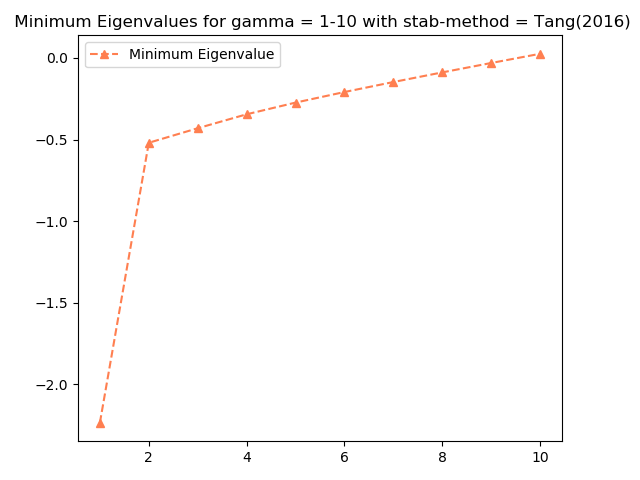
\includegraphics[width=\textwidth]{latex/Thesis/media/Gamma_1_thru_10_tang(2016)_min.png}
\caption{Minimum eigenvalues\label{fig:TangMaxEigLowMin}}
     \end{subfigure}
        \caption{Eigenvalues when using the Tangential Penalisation Max Stabilisation for \mgamma~ranging from 1 through 10}
        \label{fig:TangMaxEigLowmulti}
\end{figure}
\begin{figure}[ht]
     \centering
     \begin{subfigure}[h]{0.49\textwidth}
        \centering
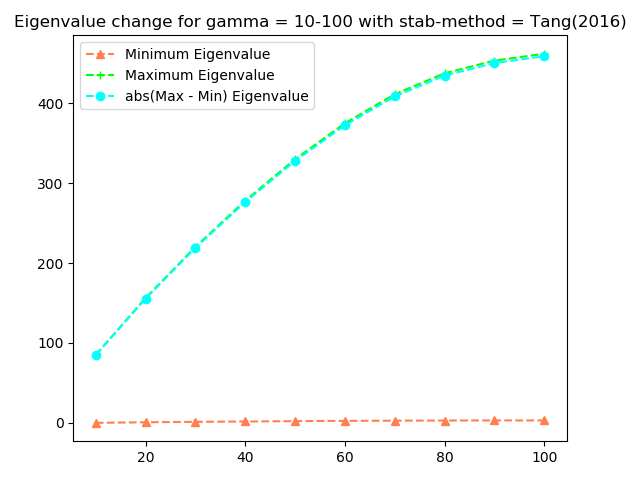
\includegraphics[width=\textwidth]{latex/Thesis/media/Gamma_10_thru_100_tang(2016).png}
\caption{Minimum and maximum eigenvalues\label{fig:TangMaxEigHigh}}
     \end{subfigure}
     \hfill
     \begin{subfigure}[h]{0.49\textwidth}
\centering
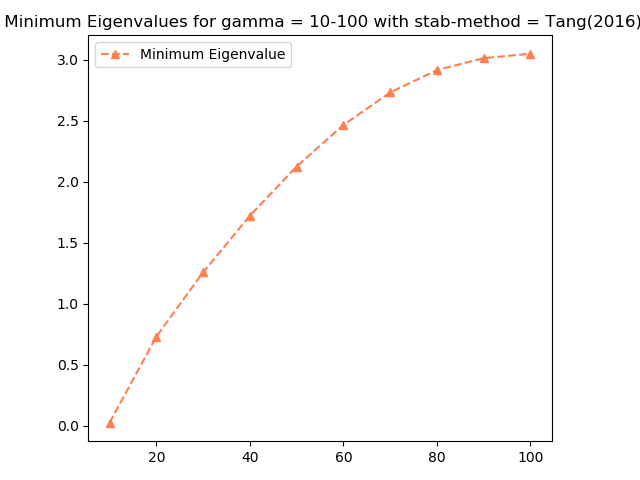
\includegraphics[width=\textwidth]{latex/Thesis/media/Gamma_10_thru_100_tang(2016)_min.png}
\caption{Minimum eigenvalues\label{fig:TangMaxEigHighMin}}
     \end{subfigure}
        \caption{Eigenvalues when using the Tangential Penalisation Max Stabilisation for \mgamma~ranging from 10 through 100}
        \label{fig:TangMaxEigHighmulti}
\end{figure}



\subsection{Tangential Penalisation}

The final stabilisation method to be considered is the Tangential Penalisation method as defined in \autoref{eq:stabTangPen} which has not been proven to have a value of \mgamma such that stability is guaranteed, so it would greatly benefit from automation. From \autoref{fig:TangEigLowmulti} it would appear to have similar behaviour to that of \autoref{fig:TangMaxEigLowmulti} however we cannot make any conclusive findings. It is when we go to \autoref{fig:TangEigHighmulti} that we observe the problem that no matter how large we are taking \mgamma, we are unable to push the minimum eigenvalue to be positive, rather it always remains negative. This requires further investigation why there is always a single eigenvalue that will not be made positive and if there are methods that could be employed that might solve this issue, such as employing pole placement.
\begin{figure}[ht]
     \centering
     \begin{subfigure}[h]{0.49\textwidth}
        \centering
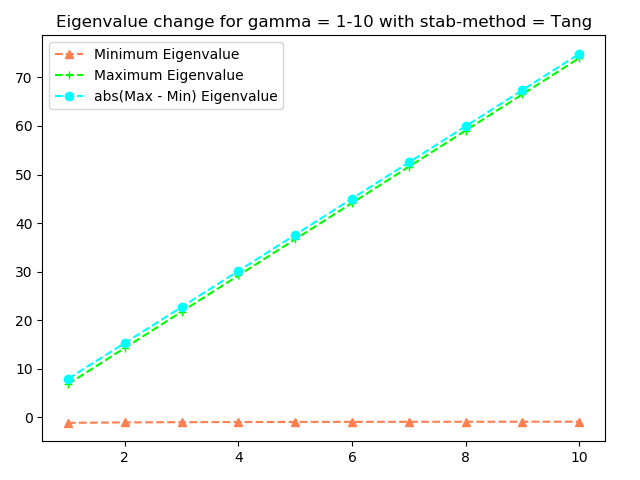
\includegraphics[width=\textwidth]{latex/Thesis/media/Gamma_1_thru_10_tang.png}
\caption{Minimum and maximum eigenvalues\label{fig:TangEigLow}}
     \end{subfigure}
     \hfill
     \begin{subfigure}[h]{0.49\textwidth}
\centering
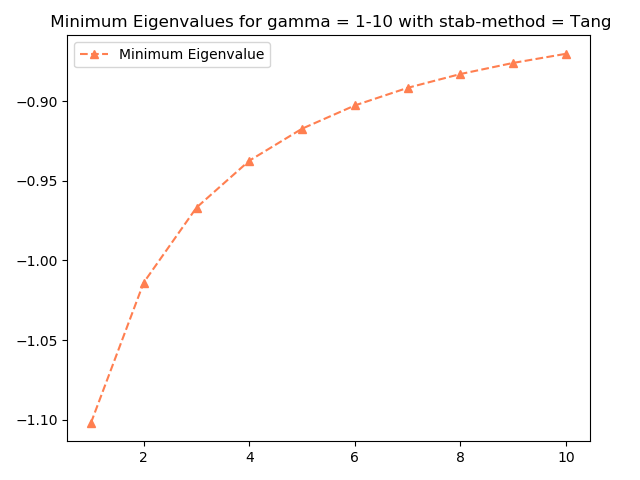
\includegraphics[width=\textwidth]{latex/Thesis/media/Gamma_1_thru_10_tang_min.png}
\caption{Minimum eigenvalues\label{fig:TangEigLowMin}}
     \end{subfigure}
        \caption{Eigenvalues when using the Tangential Penalisation Stabilisation for \mgamma~ranging from 1 through 10}
        \label{fig:TangEigLowmulti}
\end{figure}
\begin{figure}[ht]
     \centering
     \begin{subfigure}[h]{0.49\textwidth}
        \centering
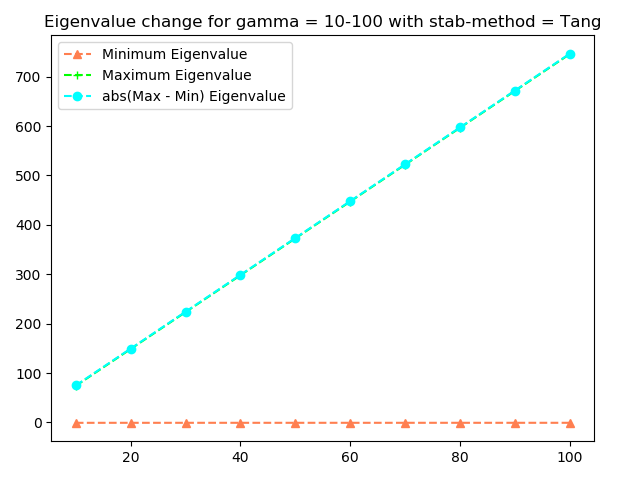
\includegraphics[width=\textwidth]{latex/Thesis/media/Gamma_10_thru_100_tang.png}
\caption{Minimum and maximum eigenvalues\label{fig:TangEigHigh}}
     \end{subfigure}
     \hfill
     \begin{subfigure}[h]{0.49\textwidth}
\centering
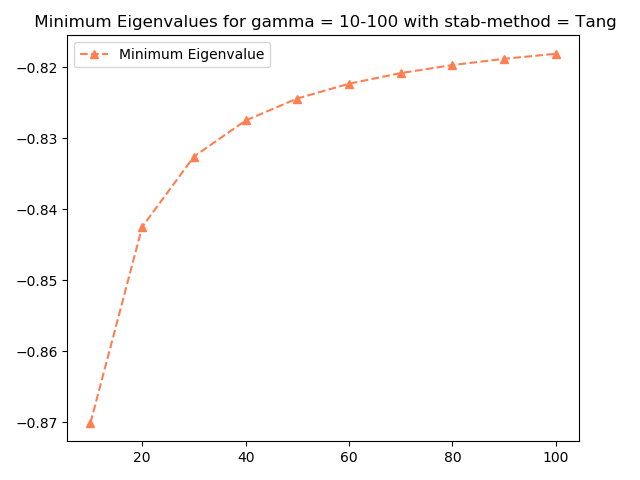
\includegraphics[width=\textwidth]{latex/Thesis/media/Gamma_10_thru_100_tang_min.png}
\caption{Minimum eigenvalues\label{fig:TangEigHighMin}}
     \end{subfigure}
        \caption{Eigenvalues when using the Tangential Penalisation Stabilisation for \mgamma~ranging from 10 through 100}
        \label{fig:TangEigHighmulti}
\end{figure}


% \subsection{Stabilisation makes eigenvalues positive}

% \subsection{Paraview plots}

